In this section, an overview of the system is given.
This does not include details about the path tracing technique, but focuses on how the system parallellizes this on the cloud.

\subsection{Dividing tasks}
Whenever a worker node $w_i$ connects to the master node $M$, the master node will add $w_i$ to its set of available worker nodes: $A$.
Any worker node that is not available, because it was assigned a task and has not finished it yet, is moved from $A$ to $W$, the set of working workers.

\begin{figure}[ht!]
    \center
    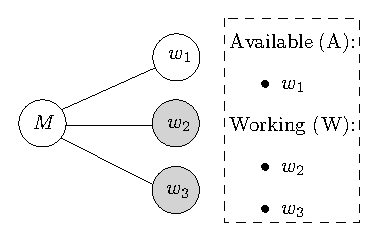
\includegraphics{./img/masterworkerconnections.eps}
    \caption{Connected workers and their set}
    \label{fig:masterworkerconnections}
\end{figure}

When $M$ receives a job $j_i$, which corresponds to a movie that needs to be rendered, $M$ splits it into a set of tasks $T = \{t_{i,1}, t_{i,2}, \ldots, t_{i,n}\}$.
Every task corresponds to a frame of the movie.
The system can receive a job from any user at any point in time and, therefore, supports multitenancy.

When receiving a job, nothing is known about the time required to process it.
Splitting it up into smaller tasks and dividing them over the assigned worker nodes balances the load of a job over multiple workers.


\begin{figure}[ht!]
    \center
    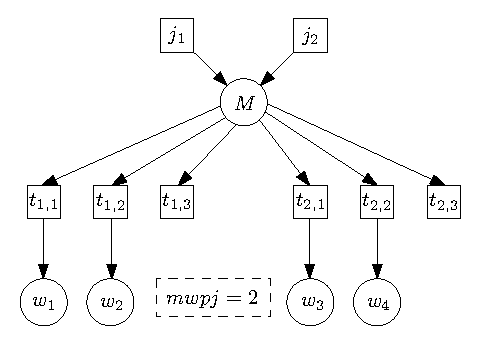
\includegraphics{./img/splitjobtotasks.eps}
    \caption{Jobs split into tasks and assigned to workers}
    \label{fig:splitjobtotasks}
\end{figure}

The system has a maximum number of worker nodes per job, $mwpj$.
This is to enable easy scaling up of the number of working workers when multiple jobs arrive, and scaling back down when demand decreases.
$mwpj$'s effect can be seen in Figure~\ref{fig:splitjobtotasks}.

\subsection{Dividing workers over jobs}
Suppose that we have $k$ jobs, $mwpj = 2$, the total amount of workers is $|A| + |W|$ and we have:
\begin{align}|A|+|W| < k \cdot mwpj \label{eq:fewWorkers}\end{align}
Now, we cannot provide every running job with its maximal amount of workers.
This is when the system switches to a different scheme.
Whenever a worker has finished its task, it will be assigned a task from the job that has not had a worker assigned to it the longest.
If that job already has $mwpj$ workers on it, then the next job in line will receive the worker, and so on.
Since Equation~\ref{eq:fewWorkers} holds, there is guaranteed to be a job in line without $mwpj$ workers already assigned to it.
This way, some fairness is created in the amount of processing time that each job gets assigned.